\documentclass{article}
\usepackage[T1]{fontenc}
\usepackage{lmodern}
\usepackage{graphicx}
\usepackage{amsmath,amssymb}
\usepackage[a4paper,margin=2cm]{geometry}
\usepackage[absolute,overlay]{textpos}
\setlength{\TPHorizModule}{1mm}
\setlength{\TPVertModule}{1mm}
\usepackage[indonesian]{babel}
\usepackage{hyperref}
\setlength{\emergencystretch}{2em}
% unit: Halaman 26

\begin{document}

% === Halaman 26 (llm) ===

\vspace{213.84mm}

Alternatif grafik lainnya:

% deskripsi: Grafik garis yang menunjukkan Jumlah Penderita Demam Berdarah di Kota Bogor dari Januari 2017 hingga Agustus 2018, dengan fluktuasi jumlah kasus per bulan.
% bbox normalisasi: [0.1700, 0.2000, 0.8200, 0.9200]
\begin{textblock*}{136.50mm}(35.70mm,59.40mm)
\noindent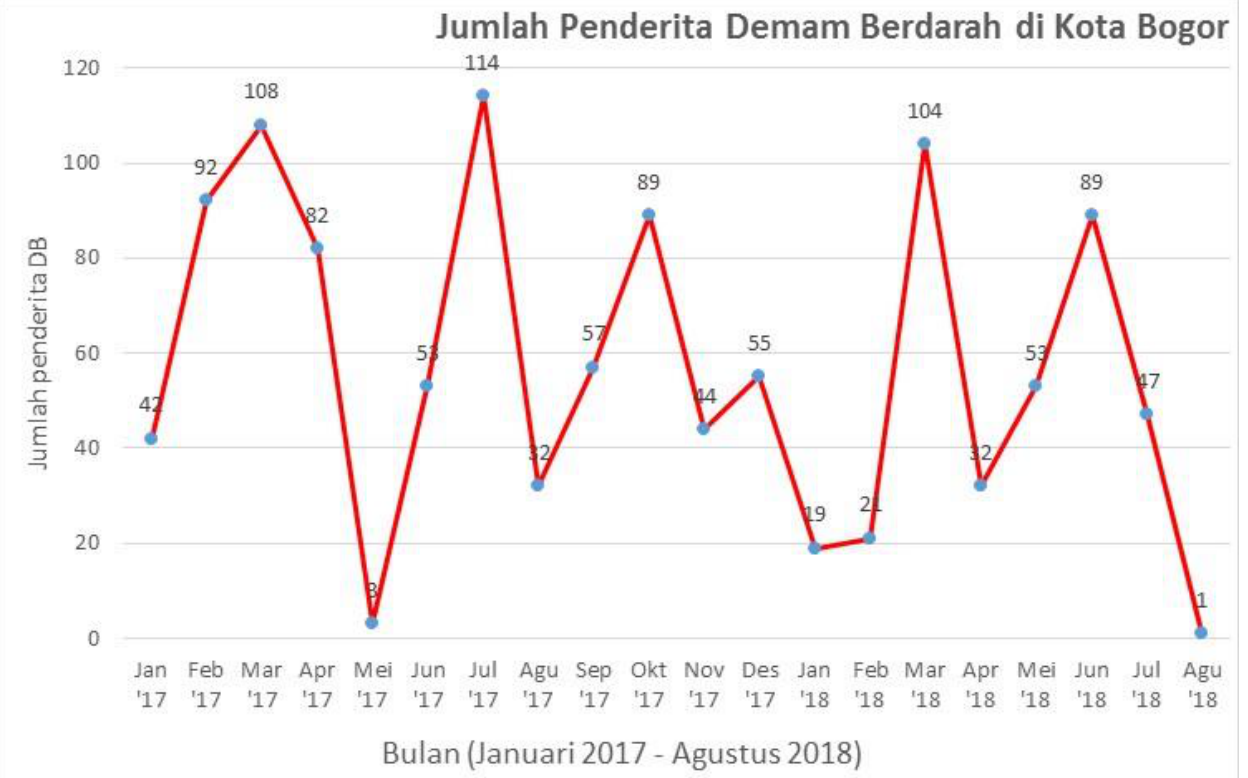
\includegraphics[width=136.50mm,height=213.84mm]{../../images/llm/page_026_img_01.png}%
\end{textblock*}

\end{document}
